% Created 2014-05-08 Thu 14:59
\documentclass[11pt]{article}
\usepackage[utf8]{inputenc}
\usepackage[T1]{fontenc}
\usepackage{fixltx2e}
\usepackage{graphicx}
\usepackage{longtable}
\usepackage{float}
\usepackage{wrapfig}
\usepackage{rotating}
\usepackage[normalem]{ulem}
\usepackage{amsmath}
\usepackage{textcomp}
\usepackage{marvosym}
\usepackage{wasysym}
\usepackage{amssymb}
\usepackage{hyperref}
\tolerance=1000
\author{James Woodward Weis}
\date{\today}
\title{Compiled Biological Knowledge}
\hypersetup{
  pdfkeywords={},
  pdfsubject={},
  pdfcreator={Emacs 24.3.1 (Org mode 8.2.4)}}
\begin{document}

\maketitle
\tableofcontents


\section{Hallmarks of cancer}
\label{sec-1}

\subsection{Six original hallmarks of cancer}
\label{sec-1-1}
\begin{enumerate}
\item Sustain Proliferative Signaling
\item Evading Growth Suppressors
\item Resisting Cell Death
\item Enabling Replicative Immorality
\item Inducing Angiogenesis
\item Activating Invasion and Metastasis
\end{enumerate}
\subsection{Additional "enabling" and "emerging" hallmarks}
\label{sec-1-2}
\begin{enumerate}
\item Enabling: Genome instability and mutation
\item Enabling: Tumor-promoting inflammation
\item Emerging: Reprogramming energy metabolism
\item Emerging: Evading immune destruction
\end{enumerate}
\section{Intracellular circuitry of relevance in cancer}
\label{sec-2}
\begin{figure}[htb]
\centering
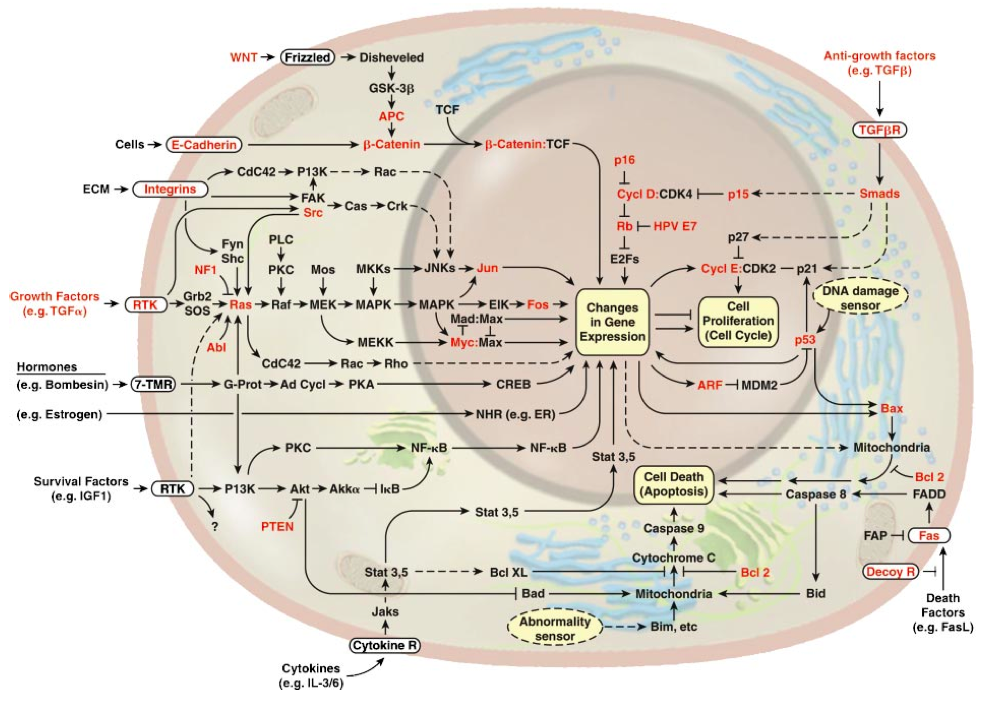
\includegraphics[width=.9\linewidth]{./BIO-KNOWLEDGE-DIAGRAM.png}
\caption{Diagram of biological knowledge dataset.o}
\end{figure}

Circuit 'outputs' or results:
\begin{itemize}
\item Gene Expression
\item Cell Proliferation (Cell cycle)
\item Cell Death (Apoptosis)
\end{itemize}

Circuit non-molecular inputs:
\begin{itemize}
\item DNA Damage Sensor
\item Abnormality Sensor
\item Other cells
\end{itemize}

Note that in the following subsections, an \uline{underline} indicates an alias for a family of molecules, while \textbf{bold} indicates a non-molecular input or output.

\subsection{Wnt signaling pathway}
\label{sec-2-1}
Relations:
\begin{itemize}
\item WNT + Frizzled -> WNT:Frizzled
\item WNT:Frizzled -> Dishevelled
\item Dishevelled -> GSK-3Beta
\item GSK-3Beta -> APC
\item APC -> Beta-Cetenin
\item \uline{Other-cell} + E-Cadherin -> Beta-Catenin
\item Beta-Catenin + TCF -> Beta-Catenin:TCF
\item Beta-Catenin:TCF -> \textbf{Changes-in-Gene-Expression}
\end{itemize}
\subsection{TGF-Beta Pathway}
\label{sec-2-2}
Relations:
\begin{itemize}
\item TGF-Beta + TGF-Beta-R -> TGF-Beta:TGF-Beta-R
\item TGF-Beta:TGF-Beta-R -> \uline{SMADs}

\item \uline{SMADs} -> p15
\item Cyclin-D + CDK4 -> Cyclin-D:CDK4
\item p16 -| Cyclin-D:CDK4
\item p15 -| Cyclin-D:CDK4
\item Cyclin-D:CDK4 -| Rb
\item HPV-E7 -| Rb
\item Rb -| \uline{E2Fs}
\item \uline{E2Fs} -| \textbf{Changes-in-gene-expression}

\item \uline{SMADs} -> p27
\item Cyclin-E + CDK2 -> Cyclin-E:CDK2
\item p27 -| Cyclin-E:CDK2
\item Cyclin-E:CDK2 -> \textbf{Cell-Proliferation}
\item \textbf{Changes-in-gene-expression} -> Cyclin-E:CDK2

\item \uline{SMADs} -> p21
\item Cyclin-E + CDK2 -> Cyclin-E:CDK2
\item p21 -| Cyclin-E:CDK2
\end{itemize}
\subsection{DNA Damage sensing pathway}
\label{sec-2-3}

Relations:
\begin{itemize}
\item p53 -> p21
\item p53 -> Bax
\item p53 -> \textbf{Changes-in-gene-expression}
\item \textbf{Changes-in-gene-expression} -> ARF
\item ARF -| MDM2
\item MDM2 -| p53
\item Bax -> Mitochondria
\item Mitochondria + (not Bcl2) -> \textbf{Apoptosis}
\end{itemize}
\subsection{Death factor pathway}
\label{sec-2-4}
Relations:
\begin{itemize}
\item FasL + Fas + (not FAP) + (not Decoy-Fas) -> FADD
\item FADD -> Caspase8
\item Caspase8 -> Bid
\item Caspase8 -> \textbf{Apoptosis}
\item Bid -> Mitochondria
\item \textbf{Abnormality-sensor} -> Bim
\item Bim -> Mitochondria
\item Mitochondria + (not Bcl2) + (not BclXL) -> CytochromeC
\item CytochromeC -> Caspase9
\item Caspase9 -> \textbf{Apoptosis}
\end{itemize}
\subsection{Cytokine Pathway}
\label{sec-2-5}
Relations:
\begin{itemize}
\item \uline{Cytokines} + Cytokine-R -> \uline{Jaks}
\item \uline{Jaks} -> Stat3
\item \uline{Jaks} -> Stat5
\item Stat3 -> BclXL
\item Stat5 -> BclXL
\item Stat3 -> \textbf{Changes-in-gene-expression}
\item Stat5 -> \textbf{Changes-in-gene-expression}
\end{itemize}
\subsection{Survival Factor Pathway}
\label{sec-2-6}
Relations:
\begin{itemize}
\item \uline{Survival-factors} + RTK -> P13K
\item \uline{Survival-factors} + RTK -> Ras
\item P13K -> Akt
\item PTEN -| Akt
\item Akt -> Akk-alpha
\item Akk-alpha -| IkB
\item IkB -> NF-KB
\item P13K -> PKC
\item PKC -> NF-KB
\item NF-KB -> \textbf{Changes-in-gene-expression}
\end{itemize}
\subsection{Hormone Pathway}
\label{sec-2-7}
Relations:
\begin{itemize}
\item Estrogen -> ER
\item ER -> \textbf{Changes-in-gene-expression}
\item Bombesin + 7-TMR -> G-Protein
\item G-Protein -> Ad-Cyclin
\item Ad-Cyclin -> PKA
\item PKA -> CREB
\item CREB -> \textbf{Changes-in-gene-expression}
\end{itemize}
\subsection{Growth factor pathway}
\label{sec-2-8}
Relations:
\begin{itemize}
\item TGF-alpha + RTK -> Grb2
\item TGF-alpha + RTK -> Src
\item TGF-alpha + RTK -> SOS
\item Grb2 -> Ras
\item SOS -> Ras
\item NF1 -| Ras
\item Abl -| Ras
\item Fyn -> Ras
\item Shc -> Ras
\item Src -> Ras
\item Ras -> Raf
\item Ras -> CdC42
\item PLC -> PKC
\item PKC -> Raf
\item CdC42 -> Rac
\item Rac -> Rho
\item Rho -> \textbf{Changes-in-gene-expression}
\item Raf -> MEK
\item Mos -> MEK
\item MEK -> MEKK
\item MEK -> MAPK
\item MAPK -> EIK
\item EIK -> Fos
\item Fos -> \textbf{Changes-in-gene-expression}
\item MAPK -> Myc:Max
\item MEKK -> Myc:Max
\item Myc + Max -> Myx:Max
\item Mad + Max -> Mad:Max
\item Myc:Max -| Mad:Max
\item Mad:Max -| Myc:Max
\item \uline{MKKs} -> MAPK
\item \uline{MKKs} -> \uline{JNKs}
\item \uline{JNKs} -> Jun
\item Jun -> \textbf{Changes-in-gene-expression}
\item MAPK -> Jun
\end{itemize}
\subsection{ECM Pathway}
\label{sec-2-9}
\begin{itemize}
\item ECM + \uline{Integrins} -> FAK
\item ECM + \uline{Integrins} -> CdC42
\item ECM + \uline{Integrins} -> Fyn
\item CdC42 -> P13K
\item P13K -> Rac
\item Rac -> \uline{JKKs}
\item FAK -> P13K
\item FAK -> Cas
\item Cas -> Crk
\item Crk -> \uline{JKKs}
\end{itemize}






\section{References}
\label{sec-3}
\begin{itemize}
\item Hanahan, D., and Weinberg, R.A. (2000). The Hallmarks of Cancer. Cell 100, 57-70.
\item Hanahan, D., and Weinberg, R.A. (2011). The Hallmarks of Cancer: The Next Generation. Cell 144, 646-674.
\item Heldin, C., Miayazono, K., and Dijke, P. (1997). TGF-Beta signalling from cell membreane to nucleus through SMAD proteins.
\item Huelsken, J., and Juergen, B. (2000). The Wnt signalling pathway. J. Cell Sci. 113, 3545.
\item Muller, H., et al. (2001). E2Fs regulate the expression of genes involved in differentiation, development, proliferation, and apoptosis. Genes Dev., 15(3): 257-285.
\end{itemize}
% Emacs 24.3.1 (Org mode 8.2.4)
\end{document}